\documentclass[twoside]{book}

% Packages required by doxygen
\usepackage{fixltx2e}
\usepackage{calc}
\usepackage{doxygen}
\usepackage[export]{adjustbox} % also loads graphicx
\usepackage{graphicx}
\usepackage[utf8]{inputenc}
\usepackage{makeidx}
\usepackage{multicol}
\usepackage{multirow}
\PassOptionsToPackage{warn}{textcomp}
\usepackage{textcomp}
\usepackage[nointegrals]{wasysym}
\usepackage[table]{xcolor}

% Font selection
\usepackage[T1]{fontenc}
\usepackage[scaled=.90]{helvet}
\usepackage{courier}
\usepackage{amssymb}
\usepackage{sectsty}
\renewcommand{\familydefault}{\sfdefault}
\allsectionsfont{%
  \fontseries{bc}\selectfont%
  \color{darkgray}%
}
\renewcommand{\DoxyLabelFont}{%
  \fontseries{bc}\selectfont%
  \color{darkgray}%
}
\newcommand{\+}{\discretionary{\mbox{\scriptsize$\hookleftarrow$}}{}{}}

% Page & text layout
\usepackage{geometry}
\geometry{%
  a4paper,%
  top=2.5cm,%
  bottom=2.5cm,%
  left=2.5cm,%
  right=2.5cm%
}
\tolerance=750
\hfuzz=15pt
\hbadness=750
\setlength{\emergencystretch}{15pt}
\setlength{\parindent}{0cm}
\setlength{\parskip}{3ex plus 2ex minus 2ex}
\makeatletter
\renewcommand{\paragraph}{%
  \@startsection{paragraph}{4}{0ex}{-1.0ex}{1.0ex}{%
    \normalfont\normalsize\bfseries\SS@parafont%
  }%
}
\renewcommand{\subparagraph}{%
  \@startsection{subparagraph}{5}{0ex}{-1.0ex}{1.0ex}{%
    \normalfont\normalsize\bfseries\SS@subparafont%
  }%
}
\makeatother

% Headers & footers
\usepackage{fancyhdr}
\pagestyle{fancyplain}
\fancyhead[LE]{\fancyplain{}{\bfseries\thepage}}
\fancyhead[CE]{\fancyplain{}{}}
\fancyhead[RE]{\fancyplain{}{\bfseries\leftmark}}
\fancyhead[LO]{\fancyplain{}{\bfseries\rightmark}}
\fancyhead[CO]{\fancyplain{}{}}
\fancyhead[RO]{\fancyplain{}{\bfseries\thepage}}
\fancyfoot[LE]{\fancyplain{}{}}
\fancyfoot[CE]{\fancyplain{}{}}
\fancyfoot[RE]{\fancyplain{}{\bfseries\scriptsize Generated by Doxygen }}
\fancyfoot[LO]{\fancyplain{}{\bfseries\scriptsize Generated by Doxygen }}
\fancyfoot[CO]{\fancyplain{}{}}
\fancyfoot[RO]{\fancyplain{}{}}
\renewcommand{\footrulewidth}{0.4pt}
\renewcommand{\chaptermark}[1]{%
  \markboth{#1}{}%
}
\renewcommand{\sectionmark}[1]{%
  \markright{\thesection\ #1}%
}

% Indices & bibliography
\usepackage{natbib}
\usepackage[titles]{tocloft}
\setcounter{tocdepth}{3}
\setcounter{secnumdepth}{5}
\makeindex

% Hyperlinks (required, but should be loaded last)
\usepackage{ifpdf}
\ifpdf
  \usepackage[pdftex,pagebackref=true]{hyperref}
\else
  \usepackage[ps2pdf,pagebackref=true]{hyperref}
\fi
\hypersetup{%
  colorlinks=true,%
  linkcolor=blue,%
  citecolor=blue,%
  unicode%
}

% Custom commands
\newcommand{\clearemptydoublepage}{%
  \newpage{\pagestyle{empty}\cleardoublepage}%
}

\usepackage{caption}
\captionsetup{labelsep=space,justification=centering,font={bf},singlelinecheck=off,skip=4pt,position=top}

%===== C O N T E N T S =====

\begin{document}

% Titlepage & ToC
\hypersetup{pageanchor=false,
             bookmarksnumbered=true,
             pdfencoding=unicode
            }
\pagenumbering{roman}
\begin{titlepage}
\vspace*{7cm}
\begin{center}%
{\Large mtmn }\\
\vspace*{1cm}
{\large Generated by Doxygen 1.8.11}\\
\end{center}
\end{titlepage}
\clearemptydoublepage
\tableofcontents
\clearemptydoublepage
\pagenumbering{arabic}
\hypersetup{pageanchor=true}

%--- Begin generated contents ---
\chapter{Data Structure Index}
\section{Data Structures}
Here are the data structures with brief descriptions\+:\begin{DoxyCompactList}
\item\contentsline{section}{\hyperlink{structmtmn__net__t}{mtmn\+\_\+net\+\_\+t} }{\pageref{structmtmn__net__t}}{}
\item\contentsline{section}{\hyperlink{structnet__config__t}{net\+\_\+config\+\_\+t} }{\pageref{structnet__config__t}}{}
\end{DoxyCompactList}

\chapter{File Index}
\section{File List}
Here is a list of all files with brief descriptions\+:\begin{DoxyCompactList}
\item\contentsline{section}{/home/yehangyang/\+Documents/\+Gitlab/others/esp-\/face/face\+\_\+detection/mtmn/include/\hyperlink{face__detection__forward_8h}{face\+\_\+detection\+\_\+forward.\+h} }{\pageref{face__detection__forward_8h}}{}
\item\contentsline{section}{/home/yehangyang/\+Documents/\+Gitlab/others/esp-\/face/face\+\_\+detection/mtmn/include/\hyperlink{mtmn_8h}{mtmn.\+h} }{\pageref{mtmn_8h}}{}
\end{DoxyCompactList}

\chapter{Data Structure Documentation}
\hypertarget{structmtmn__net__t}{}\section{mtmn\+\_\+net\+\_\+t Struct Reference}
\label{structmtmn__net__t}\index{mtmn\+\_\+net\+\_\+t@{mtmn\+\_\+net\+\_\+t}}


{\ttfamily \#include $<$mtmn.\+h$>$}

\subsection*{Data Fields}
\begin{DoxyCompactItemize}
\item 
dl\+\_\+matrix3d\+\_\+t $\ast$ \hyperlink{structmtmn__net__t_a1d3531c1210c49940c846cd600b6d2f8}{category}
\item 
dl\+\_\+matrix3d\+\_\+t $\ast$ \hyperlink{structmtmn__net__t_a0903a36fc3368901a05211a31007653b}{offset}
\item 
dl\+\_\+matrix3d\+\_\+t $\ast$ \hyperlink{structmtmn__net__t_a47e72642944e5a6a519942b74c540aec}{landmark}
\end{DoxyCompactItemize}


\subsection{Field Documentation}
\index{mtmn\+\_\+net\+\_\+t@{mtmn\+\_\+net\+\_\+t}!category@{category}}
\index{category@{category}!mtmn\+\_\+net\+\_\+t@{mtmn\+\_\+net\+\_\+t}}
\subsubsection[{\texorpdfstring{category}{category}}]{\setlength{\rightskip}{0pt plus 5cm}dl\+\_\+matrix3d\+\_\+t$\ast$ category}\hypertarget{structmtmn__net__t_a1d3531c1210c49940c846cd600b6d2f8}{}\label{structmtmn__net__t_a1d3531c1210c49940c846cd600b6d2f8}
\index{mtmn\+\_\+net\+\_\+t@{mtmn\+\_\+net\+\_\+t}!landmark@{landmark}}
\index{landmark@{landmark}!mtmn\+\_\+net\+\_\+t@{mtmn\+\_\+net\+\_\+t}}
\subsubsection[{\texorpdfstring{landmark}{landmark}}]{\setlength{\rightskip}{0pt plus 5cm}dl\+\_\+matrix3d\+\_\+t$\ast$ landmark}\hypertarget{structmtmn__net__t_a47e72642944e5a6a519942b74c540aec}{}\label{structmtmn__net__t_a47e72642944e5a6a519942b74c540aec}
\index{mtmn\+\_\+net\+\_\+t@{mtmn\+\_\+net\+\_\+t}!offset@{offset}}
\index{offset@{offset}!mtmn\+\_\+net\+\_\+t@{mtmn\+\_\+net\+\_\+t}}
\subsubsection[{\texorpdfstring{offset}{offset}}]{\setlength{\rightskip}{0pt plus 5cm}dl\+\_\+matrix3d\+\_\+t$\ast$ offset}\hypertarget{structmtmn__net__t_a0903a36fc3368901a05211a31007653b}{}\label{structmtmn__net__t_a0903a36fc3368901a05211a31007653b}


The documentation for this struct was generated from the following file\+:\begin{DoxyCompactItemize}
\item 
/home/yehangyang/\+Documents/\+Gitlab/others/esp-\/face/face\+\_\+detection/mtmn/include/\hyperlink{mtmn_8h}{mtmn.\+h}\end{DoxyCompactItemize}

\hypertarget{structnet__config__t}{}\section{net\+\_\+config\+\_\+t Struct Reference}
\label{structnet__config__t}\index{net\+\_\+config\+\_\+t@{net\+\_\+config\+\_\+t}}


{\ttfamily \#include $<$mtmn.\+h$>$}

\subsection*{Data Fields}
\begin{DoxyCompactItemize}
\item 
\hyperlink{mtmn_8h_a9eb3d74ee60112199ec78344b3a4655e}{net\+\_\+type\+\_\+en} \hyperlink{structnet__config__t_a8f4c2af8911d60345894c9b1cd728a81}{net\+\_\+type}
\item 
char $\ast$ \hyperlink{structnet__config__t_a8505c513bc640d1f69e5f76fb32b24a8}{file\+\_\+name}
\item 
int \hyperlink{structnet__config__t_aac374e320caaadeca4874add33b62af2}{w}
\item 
int \hyperlink{structnet__config__t_a16611451551e3d15916bae723c3f59f7}{h}
\item 
float \hyperlink{structnet__config__t_ace479cfe5e33dac6639cf88d0551b58c}{score\+\_\+threshold}
\item 
float \hyperlink{structnet__config__t_a363bfab5175aae09f069a69ff5072f2c}{nms\+\_\+threshold}
\end{DoxyCompactItemize}


\subsection{Field Documentation}
\index{net\+\_\+config\+\_\+t@{net\+\_\+config\+\_\+t}!file\+\_\+name@{file\+\_\+name}}
\index{file\+\_\+name@{file\+\_\+name}!net\+\_\+config\+\_\+t@{net\+\_\+config\+\_\+t}}
\subsubsection[{\texorpdfstring{file\+\_\+name}{file_name}}]{\setlength{\rightskip}{0pt plus 5cm}char$\ast$ file\+\_\+name}\hypertarget{structnet__config__t_a8505c513bc640d1f69e5f76fb32b24a8}{}\label{structnet__config__t_a8505c513bc640d1f69e5f76fb32b24a8}
\index{net\+\_\+config\+\_\+t@{net\+\_\+config\+\_\+t}!h@{h}}
\index{h@{h}!net\+\_\+config\+\_\+t@{net\+\_\+config\+\_\+t}}
\subsubsection[{\texorpdfstring{h}{h}}]{\setlength{\rightskip}{0pt plus 5cm}int h}\hypertarget{structnet__config__t_a16611451551e3d15916bae723c3f59f7}{}\label{structnet__config__t_a16611451551e3d15916bae723c3f59f7}
\index{net\+\_\+config\+\_\+t@{net\+\_\+config\+\_\+t}!net\+\_\+type@{net\+\_\+type}}
\index{net\+\_\+type@{net\+\_\+type}!net\+\_\+config\+\_\+t@{net\+\_\+config\+\_\+t}}
\subsubsection[{\texorpdfstring{net\+\_\+type}{net_type}}]{\setlength{\rightskip}{0pt plus 5cm}{\bf net\+\_\+type\+\_\+en} net\+\_\+type}\hypertarget{structnet__config__t_a8f4c2af8911d60345894c9b1cd728a81}{}\label{structnet__config__t_a8f4c2af8911d60345894c9b1cd728a81}
\index{net\+\_\+config\+\_\+t@{net\+\_\+config\+\_\+t}!nms\+\_\+threshold@{nms\+\_\+threshold}}
\index{nms\+\_\+threshold@{nms\+\_\+threshold}!net\+\_\+config\+\_\+t@{net\+\_\+config\+\_\+t}}
\subsubsection[{\texorpdfstring{nms\+\_\+threshold}{nms_threshold}}]{\setlength{\rightskip}{0pt plus 5cm}float nms\+\_\+threshold}\hypertarget{structnet__config__t_a363bfab5175aae09f069a69ff5072f2c}{}\label{structnet__config__t_a363bfab5175aae09f069a69ff5072f2c}
\index{net\+\_\+config\+\_\+t@{net\+\_\+config\+\_\+t}!score\+\_\+threshold@{score\+\_\+threshold}}
\index{score\+\_\+threshold@{score\+\_\+threshold}!net\+\_\+config\+\_\+t@{net\+\_\+config\+\_\+t}}
\subsubsection[{\texorpdfstring{score\+\_\+threshold}{score_threshold}}]{\setlength{\rightskip}{0pt plus 5cm}float score\+\_\+threshold}\hypertarget{structnet__config__t_ace479cfe5e33dac6639cf88d0551b58c}{}\label{structnet__config__t_ace479cfe5e33dac6639cf88d0551b58c}
\index{net\+\_\+config\+\_\+t@{net\+\_\+config\+\_\+t}!w@{w}}
\index{w@{w}!net\+\_\+config\+\_\+t@{net\+\_\+config\+\_\+t}}
\subsubsection[{\texorpdfstring{w}{w}}]{\setlength{\rightskip}{0pt plus 5cm}int w}\hypertarget{structnet__config__t_aac374e320caaadeca4874add33b62af2}{}\label{structnet__config__t_aac374e320caaadeca4874add33b62af2}


The documentation for this struct was generated from the following file\+:\begin{DoxyCompactItemize}
\item 
/home/yehangyang/\+Documents/\+Gitlab/others/esp-\/face/face\+\_\+detection/mtmn/include/\hyperlink{mtmn_8h}{mtmn.\+h}\end{DoxyCompactItemize}

\chapter{File Documentation}
\hypertarget{face__detection__forward_8h}{}\section{/home/yehangyang/\+Documents/\+Gitlab/others/esp-\/face/face\+\_\+detection/mtmn/include/face\+\_\+detection\+\_\+forward.h File Reference}
\label{face__detection__forward_8h}\index{/home/yehangyang/\+Documents/\+Gitlab/others/esp-\/face/face\+\_\+detection/mtmn/include/face\+\_\+detection\+\_\+forward.\+h@{/home/yehangyang/\+Documents/\+Gitlab/others/esp-\/face/face\+\_\+detection/mtmn/include/face\+\_\+detection\+\_\+forward.\+h}}
{\ttfamily \#include \char`\"{}image\+\_\+util.\+h\char`\"{}}\\*
{\ttfamily \#include \char`\"{}dl\+\_\+lib.\+h\char`\"{}}\\*
Include dependency graph for face\+\_\+detection\+\_\+forward.\+h\+:\nopagebreak
\begin{figure}[H]
\begin{center}
\leavevmode
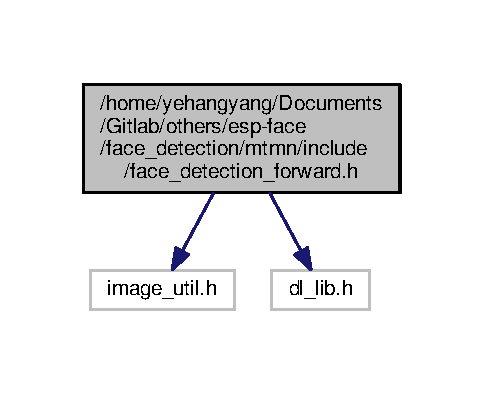
\includegraphics[width=232pt]{face__detection__forward_8h__incl}
\end{center}
\end{figure}
\subsection*{Macros}
\begin{DoxyCompactItemize}
\item 
\#define \hyperlink{face__detection__forward_8h_a20978e37cee4ae0da7b405df9fd15b7d}{M\+A\+X\+\_\+\+D\+E\+T\+E\+C\+T\+I\+ON}~1
\end{DoxyCompactItemize}
\subsection*{Functions}
\begin{DoxyCompactItemize}
\item 
box\+\_\+array\+\_\+t $\ast$ \hyperlink{face__detection__forward_8h_a38284a9b843c9c6162f17c72f0d3fa5d}{face\+\_\+detect} (dl\+\_\+matrix3du\+\_\+t $\ast$image\+\_\+matrix)
\begin{DoxyCompactList}\small\item\em Do M\+T\+MN face detection, return box and landmark infomation. \end{DoxyCompactList}\end{DoxyCompactItemize}


\subsection{Macro Definition Documentation}
\index{face\+\_\+detection\+\_\+forward.\+h@{face\+\_\+detection\+\_\+forward.\+h}!M\+A\+X\+\_\+\+D\+E\+T\+E\+C\+T\+I\+ON@{M\+A\+X\+\_\+\+D\+E\+T\+E\+C\+T\+I\+ON}}
\index{M\+A\+X\+\_\+\+D\+E\+T\+E\+C\+T\+I\+ON@{M\+A\+X\+\_\+\+D\+E\+T\+E\+C\+T\+I\+ON}!face\+\_\+detection\+\_\+forward.\+h@{face\+\_\+detection\+\_\+forward.\+h}}
\subsubsection[{\texorpdfstring{M\+A\+X\+\_\+\+D\+E\+T\+E\+C\+T\+I\+ON}{MAX_DETECTION}}]{\setlength{\rightskip}{0pt plus 5cm}\#define M\+A\+X\+\_\+\+D\+E\+T\+E\+C\+T\+I\+ON~1}\hypertarget{face__detection__forward_8h_a20978e37cee4ae0da7b405df9fd15b7d}{}\label{face__detection__forward_8h_a20978e37cee4ae0da7b405df9fd15b7d}


\subsection{Function Documentation}
\index{face\+\_\+detection\+\_\+forward.\+h@{face\+\_\+detection\+\_\+forward.\+h}!face\+\_\+detect@{face\+\_\+detect}}
\index{face\+\_\+detect@{face\+\_\+detect}!face\+\_\+detection\+\_\+forward.\+h@{face\+\_\+detection\+\_\+forward.\+h}}
\subsubsection[{\texorpdfstring{face\+\_\+detect(dl\+\_\+matrix3du\+\_\+t $\ast$image\+\_\+matrix)}{face_detect(dl_matrix3du_t *image_matrix)}}]{\setlength{\rightskip}{0pt plus 5cm}box\+\_\+array\+\_\+t$\ast$ face\+\_\+detect (
\begin{DoxyParamCaption}
\item[{dl\+\_\+matrix3du\+\_\+t $\ast$}]{image\+\_\+matrix}
\end{DoxyParamCaption}
)}\hypertarget{face__detection__forward_8h_a38284a9b843c9c6162f17c72f0d3fa5d}{}\label{face__detection__forward_8h_a38284a9b843c9c6162f17c72f0d3fa5d}


Do M\+T\+MN face detection, return box and landmark infomation. 


\begin{DoxyParams}{Parameters}
{\em image\+\_\+matrix} & Image matrix, rgb888 format \\
\hline
\end{DoxyParams}
\begin{DoxyReturn}{Returns}
box\+\_\+array\+\_\+t$\ast$ A list of boxes and score. 
\end{DoxyReturn}

\hypertarget{mtmn_8h}{}\section{/home/yehangyang/\+Documents/\+Gitlab/others/esp-\/face/face\+\_\+detection/mtmn/include/mtmn.h File Reference}
\label{mtmn_8h}\index{/home/yehangyang/\+Documents/\+Gitlab/others/esp-\/face/face\+\_\+detection/mtmn/include/mtmn.\+h@{/home/yehangyang/\+Documents/\+Gitlab/others/esp-\/face/face\+\_\+detection/mtmn/include/mtmn.\+h}}
{\ttfamily \#include \char`\"{}dl\+\_\+lib.\+h\char`\"{}}\\*
Include dependency graph for mtmn.\+h\+:\nopagebreak
\begin{figure}[H]
\begin{center}
\leavevmode
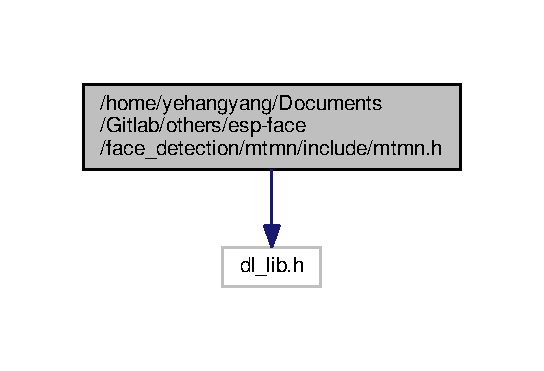
\includegraphics[width=261pt]{mtmn_8h__incl}
\end{center}
\end{figure}
\subsection*{Data Structures}
\begin{DoxyCompactItemize}
\item 
struct \hyperlink{structnet__config__t}{net\+\_\+config\+\_\+t}
\item 
struct \hyperlink{structmtmn__net__t}{mtmn\+\_\+net\+\_\+t}
\end{DoxyCompactItemize}
\subsection*{Enumerations}
\begin{DoxyCompactItemize}
\item 
enum \hyperlink{mtmn_8h_a9eb3d74ee60112199ec78344b3a4655e}{net\+\_\+type\+\_\+en} \{ \hyperlink{mtmn_8h_a9eb3d74ee60112199ec78344b3a4655ea420967c595d18a6c724a0e23758e13a3}{P\+N\+ET} = 0, 
\hyperlink{mtmn_8h_a9eb3d74ee60112199ec78344b3a4655ea04f27ba307b14f27addd295c98ddf553}{R\+N\+ET} = 1, 
\hyperlink{mtmn_8h_a9eb3d74ee60112199ec78344b3a4655eae014747eb28337b8039bd469eb6a8922}{O\+N\+ET} = 2
 \}
\end{DoxyCompactItemize}
\subsection*{Functions}
\begin{DoxyCompactItemize}
\item 
\hyperlink{structmtmn__net__t}{mtmn\+\_\+net\+\_\+t} $\ast$ \hyperlink{mtmn_8h_afac4461942a87d707bd4898dcedb29a0}{pnet} (dl\+\_\+matrix3du\+\_\+t $\ast$in)
\begin{DoxyCompactList}\small\item\em Forward the pnet process, coarse detection. \end{DoxyCompactList}\item 
\hyperlink{structmtmn__net__t}{mtmn\+\_\+net\+\_\+t} $\ast$ \hyperlink{mtmn_8h_aa313cde296f06b62ab29ec76fb415001}{rnet\+\_\+with\+\_\+score\+\_\+verify} (dl\+\_\+matrix3du\+\_\+t $\ast$in, float threshold)
\begin{DoxyCompactList}\small\item\em Forward the rnet process, fine determine the boxes from pnet. \end{DoxyCompactList}\item 
\hyperlink{structmtmn__net__t}{mtmn\+\_\+net\+\_\+t} $\ast$ \hyperlink{mtmn_8h_a34bd9533ca58ee5d4b6ff19b548c0a39}{onet\+\_\+with\+\_\+score\+\_\+verify} (dl\+\_\+matrix3du\+\_\+t $\ast$in, float threshold)
\begin{DoxyCompactList}\small\item\em Forward the onet process, fine determine the boxes from rnet. \end{DoxyCompactList}\end{DoxyCompactItemize}


\subsection{Enumeration Type Documentation}
\index{mtmn.\+h@{mtmn.\+h}!net\+\_\+type\+\_\+en@{net\+\_\+type\+\_\+en}}
\index{net\+\_\+type\+\_\+en@{net\+\_\+type\+\_\+en}!mtmn.\+h@{mtmn.\+h}}
\subsubsection[{\texorpdfstring{net\+\_\+type\+\_\+en}{net_type_en}}]{\setlength{\rightskip}{0pt plus 5cm}enum {\bf net\+\_\+type\+\_\+en}}\hypertarget{mtmn_8h_a9eb3d74ee60112199ec78344b3a4655e}{}\label{mtmn_8h_a9eb3d74ee60112199ec78344b3a4655e}
\begin{Desc}
\item[Enumerator]\par
\begin{description}
\index{P\+N\+ET@{P\+N\+ET}!mtmn.\+h@{mtmn.\+h}}\index{mtmn.\+h@{mtmn.\+h}!P\+N\+ET@{P\+N\+ET}}\item[{\em 
P\+N\+ET\hypertarget{mtmn_8h_a9eb3d74ee60112199ec78344b3a4655ea420967c595d18a6c724a0e23758e13a3}{}\label{mtmn_8h_a9eb3d74ee60112199ec78344b3a4655ea420967c595d18a6c724a0e23758e13a3}
}]\index{R\+N\+ET@{R\+N\+ET}!mtmn.\+h@{mtmn.\+h}}\index{mtmn.\+h@{mtmn.\+h}!R\+N\+ET@{R\+N\+ET}}\item[{\em 
R\+N\+ET\hypertarget{mtmn_8h_a9eb3d74ee60112199ec78344b3a4655ea04f27ba307b14f27addd295c98ddf553}{}\label{mtmn_8h_a9eb3d74ee60112199ec78344b3a4655ea04f27ba307b14f27addd295c98ddf553}
}]\index{O\+N\+ET@{O\+N\+ET}!mtmn.\+h@{mtmn.\+h}}\index{mtmn.\+h@{mtmn.\+h}!O\+N\+ET@{O\+N\+ET}}\item[{\em 
O\+N\+ET\hypertarget{mtmn_8h_a9eb3d74ee60112199ec78344b3a4655eae014747eb28337b8039bd469eb6a8922}{}\label{mtmn_8h_a9eb3d74ee60112199ec78344b3a4655eae014747eb28337b8039bd469eb6a8922}
}]\end{description}
\end{Desc}


\subsection{Function Documentation}
\index{mtmn.\+h@{mtmn.\+h}!onet\+\_\+with\+\_\+score\+\_\+verify@{onet\+\_\+with\+\_\+score\+\_\+verify}}
\index{onet\+\_\+with\+\_\+score\+\_\+verify@{onet\+\_\+with\+\_\+score\+\_\+verify}!mtmn.\+h@{mtmn.\+h}}
\subsubsection[{\texorpdfstring{onet\+\_\+with\+\_\+score\+\_\+verify(dl\+\_\+matrix3du\+\_\+t $\ast$in, float threshold)}{onet_with_score_verify(dl_matrix3du_t *in, float threshold)}}]{\setlength{\rightskip}{0pt plus 5cm}{\bf mtmn\+\_\+net\+\_\+t}$\ast$ onet\+\_\+with\+\_\+score\+\_\+verify (
\begin{DoxyParamCaption}
\item[{dl\+\_\+matrix3du\+\_\+t $\ast$}]{in, }
\item[{float}]{threshold}
\end{DoxyParamCaption}
)}\hypertarget{mtmn_8h_a34bd9533ca58ee5d4b6ff19b548c0a39}{}\label{mtmn_8h_a34bd9533ca58ee5d4b6ff19b548c0a39}


Forward the onet process, fine determine the boxes from rnet. 


\begin{DoxyParams}{Parameters}
{\em in} & Image matrix, rgb888 format \\
\hline
{\em threshold} & Score threshold to detect human face \\
\hline
\end{DoxyParams}
\begin{DoxyReturn}{Returns}
Scores for every box, box offset, and landmark with respect. 
\end{DoxyReturn}
\index{mtmn.\+h@{mtmn.\+h}!pnet@{pnet}}
\index{pnet@{pnet}!mtmn.\+h@{mtmn.\+h}}
\subsubsection[{\texorpdfstring{pnet(dl\+\_\+matrix3du\+\_\+t $\ast$in)}{pnet(dl_matrix3du_t *in)}}]{\setlength{\rightskip}{0pt plus 5cm}{\bf mtmn\+\_\+net\+\_\+t}$\ast$ pnet (
\begin{DoxyParamCaption}
\item[{dl\+\_\+matrix3du\+\_\+t $\ast$}]{in}
\end{DoxyParamCaption}
)}\hypertarget{mtmn_8h_afac4461942a87d707bd4898dcedb29a0}{}\label{mtmn_8h_afac4461942a87d707bd4898dcedb29a0}


Forward the pnet process, coarse detection. 


\begin{DoxyParams}{Parameters}
{\em in} & Image matrix, rgb888 format, size is 320x240 \\
\hline
\end{DoxyParams}
\begin{DoxyReturn}{Returns}
Scores for every pixel, and box offset with respect. 
\end{DoxyReturn}
\index{mtmn.\+h@{mtmn.\+h}!rnet\+\_\+with\+\_\+score\+\_\+verify@{rnet\+\_\+with\+\_\+score\+\_\+verify}}
\index{rnet\+\_\+with\+\_\+score\+\_\+verify@{rnet\+\_\+with\+\_\+score\+\_\+verify}!mtmn.\+h@{mtmn.\+h}}
\subsubsection[{\texorpdfstring{rnet\+\_\+with\+\_\+score\+\_\+verify(dl\+\_\+matrix3du\+\_\+t $\ast$in, float threshold)}{rnet_with_score_verify(dl_matrix3du_t *in, float threshold)}}]{\setlength{\rightskip}{0pt plus 5cm}{\bf mtmn\+\_\+net\+\_\+t}$\ast$ rnet\+\_\+with\+\_\+score\+\_\+verify (
\begin{DoxyParamCaption}
\item[{dl\+\_\+matrix3du\+\_\+t $\ast$}]{in, }
\item[{float}]{threshold}
\end{DoxyParamCaption}
)}\hypertarget{mtmn_8h_aa313cde296f06b62ab29ec76fb415001}{}\label{mtmn_8h_aa313cde296f06b62ab29ec76fb415001}


Forward the rnet process, fine determine the boxes from pnet. 


\begin{DoxyParams}{Parameters}
{\em in} & Image matrix, rgb888 format \\
\hline
{\em threshold} & Score threshold to detect human face \\
\hline
\end{DoxyParams}
\begin{DoxyReturn}{Returns}
Scores for every box, and box offset with respect. 
\end{DoxyReturn}

%--- End generated contents ---

% Index
\backmatter
\newpage
\phantomsection
\clearemptydoublepage
\addcontentsline{toc}{chapter}{Index}
\printindex

\end{document}
